\ifsvnmulti
\svnkwsave{$RepoFile: siminos/chao/dailyBlog.tex $}
\svnidlong {$HeadURL$}
{$LastChangedDate$}
{$LastChangedRevision$} {$LastChangedBy$}
\svnid{$Id$}
\fi


\chapter{Research blog}
\label{chap:blog}

$\footnotemark\footnotetext{{\tt \svnkw{RepoFile}}, rev. \svnfilerev:
 last edit by \svnFullAuthor{\svnfileauthor},
 \svnfilemonth/\svnfileday/\svnfileyear}$

\begin{description}

\item[Chao's Rules] On my
\HREF{http://chaosbook.org/~predrag/courses/PHYS-6124-10/RenminRibao.doc}
{Mao's boyscout honor} I pledge to add a substantial update on my
progress here at least twice a week, work incrementally and steadily on
drafts of my papers, and attend all physics colloquia, nonlinear physics,
math seminars, study groups, or my name be spelled the Italian way.
	\PC{the worry? Last blog entry is about Apr 19, today is July 18.
	``At least twice a week?''
		}

\item[2011-07-20 PC + CS] The above agreement has been solemnly signed
by Predrag and Chao, for the period starting after completing the qualifiers
Aug 22, and to Dec 31 2011.

\item[2011-03-16 PC]
Revolution is not a dinner party, not an essay, nor a painting, nor a
piece of embroidery. \HREF{http://www.youtube.com/watch?v=BS3QOtbW4m0}
{The revolution will not be televised}, will not be televised, will
not be televised, will not be televised. The revolution will be no re-run
brothers; \HREF{http://www.gilscottheron.com/lyrevol.html}{The
revolution will be live.}

\item[2011-03-16 PC to Ruslan, Stefan and Evangelos]
   Chao Shi,
\\ shichao116@gmail.com is starting ( rather late) to work on
   slicing and dicing Kuramoto Sivashinsky as a 1st year graduate student
   project. Hopefully we can get him to speed with your and Stefan's help
   within the next six months. At the moment he is reading parts of
   ChaosBook and our articles, but it might be wise that you teach him
   immediately how to use your KS programs and data, so we do not waste
   time on that. Chao can compute.

\item[2011-03-16 PC] Chao, please keep track of what goes on in
siminos/blog/ and siminos/lyapunov/ - you will be getting emails about
updates. There is some current excitement there concerning the `physical'
dimensionality of the \KS\ strange attractors.

\item[2011-03-17 CS to Ruslan, Stefan and Evangelos]
   Hi! Nice to meet you all. It is the first time I type something here.
   I am still reading Chapter 4. (and \rf{EllGaHoRa09}) I will catch up with
   you as soon as I can. Maybe I will have a lot of questions to consult
   you. Hope you won't bother:)

\item[2011-03-16 PC] Why reference to Ellis, Gay-Balmaz, Holm
                  and Ratiu\rf{EllGaHoRa09}?

%   Professor Cvitanovic, I still haven't found out why this blog cannot
%   display bibliography properly on my computer. But I think I will first
%   concentrate on those papers and come to deal with this later.

\item[2011-03-19 CS to PC]
%   Hi Professor Cvitanovic, I manage to make Latex work on my laptop
%   without actually knowing what actually happened, it works anyway. As I
%   tried one bibliography in last conversation.

   Yesterday I finished Chapter 4 but skipped the detail of the some
   examples. We discussed the first half of Chapter 4. Since there're
   pretty much mathematical detail and examples, we decide to break it
   into two parts. By the way, the notation of this chapter at the
   beginning is a little bit confusing and took me a while to get the
   concept of what those formulas really mean. I have some other
   questions about Chapter 4 but but now I am not used to typing math
   symbols here, I might ask you later directly or write it here if I get
   familiar with it.

\item[2011-03-21 PC] You have the dasbuch/book/chapter/*.tex source
code, you can just clip and paste formulas to here.

\item[2011-03-19 CS to PC]
Also I have a question about Example 3.2 in Chapter 3. It states that
   the choice of the coordinates of the pinball game are smart because
   they conserve the phase space volume. I don't understand this, would
   you mind explain it more specifically?

\item[2011-03-25 PC]
Glad you asked the question about choice of billiard coordinates. Please
write up the solution to \refexer{ex_birkhoff}; it's worth doing it in
class as well, a concrete example of how symplectic invariance preserves
area for each $(q,p)$ dual coordinate  pair.

\item[2011-04-19 CS] Done - I have verified in \refexer{ex_birkhoff} that
the 2-form/wedge product is conserved on the \Poincare section.


\item[2011-03-19 CS to PC]
Going from here, I am also
   wondering how to choose phase space coordinates? Does phase/state
   space coordinates have any requirement and whether conservation of
   space volume is such a requirement? What's the meaning of conservation
   of phase space requirement? In my understanding in Hamiltonian flows,
   conservation of phase space volume means conservation of energy, am I
   right?


\item[2011-03-25 PC]
Now, it is more subtle than that; time dependent flow can be symplectic, but energy is not conserved; I think Percival and D. Richards\rf{PerRich82N} (I have it in the
\HREF{http://www.cns.gatech.edu/CNS-only/LibraryCat2.htm} {CNS library}) discuss that well. Symplectic invariance is \emph{much stronger} requirement than either either energy conservation or phase-space volume conservation, see
\HREF{http://chaosbook.org/chapters/newton.pdf} {Section 7.4 Poincar\'e invariants} and \HREF{http://chaosbook.org/chapters/appendStability.pdf}
{Appendix D.4 Stability of Hamiltonian flows}:
symplectic transformations preserve area for each $(q,p)$ dual coordinate  pair.

\item[2011-03-22 PC to Chao]
This might be of interest to Adam, let him know about it:
\HREF{http://arxiv.org/abs/1103.3981}{arXiv:1103.3981},
\emph{Chains of rotational tori and filamentary structures close to high
 multiplicity periodic orbits in a 3D galactic potential},
 by Katsanikas, Patsis and Pinotsis.

They write
``
This paper discusses phase space structures encountered in the neighborhood of periodic orbits with high order multiplicity in a 3D autonomous Hamiltonian system with a potential of galactic type. We consider 4D spaces of section and we use the method of color and rotation [Patsis and Zachilas 1994] in order to visualize them. As examples we use the case of two orbits, one 2-periodic and one 7-periodic. We investigate the structure of multiple tori around them in the 4D surface of section and in addition we study the orbital behavior in the neighborhood of the corresponding simple unstable periodic orbits. By considering initially a few consequents in the neighborhood of the orbits in both cases we find a structure in the space of section, which is in direct correspondence with what is observed in a resonance zone of a 2D autonomous Hamiltonian system. However, in our 3D case we have instead of stability islands rotational tori, while the chaotic zone connecting the points of the unstable periodic orbit is replaced by filaments extending in 4D following a smooth color variation. For more intersections, the consequents of the orbit which started in the neighborhood of the unstable periodic orbit, diffuse in phase space and form a cloud that occupies a large volume surrounding the region containing the rotational tori. In this cloud the colors of the points are mixed. The same structures have been observed in the neighborhood of all m-periodic orbits we have examined in the system. This indicates a generic behavior.
''

\item[2011-03-19 CS to PC]
What do you mean by "take the Hall out of library"?:) I actually don't understand your last email.

\item[2011-03-25 PC]
Reference to Hall is in the {\em Lie police} section of Siminos
blog. It is good idea to keep reading updates of the three blogs - yours,
siminos/blog and siminos/lyapunov, they are all related to your work.

\item[2011-03-29 Ruslan]
Hi Chao.  If you want to use Matlab for your explorations of the \KS, then all my Matlab files can be found in /siminos/chao/matlab/ruslan.  File ksdupo.m is the primary file.  I'm using the cells feature of Matlab, so this file contains many sections that can be run independently.  There is not much in the way of comments, so you'll have to work it out for yourself.  I'll be happy to guide you through it if you ask specific questions.

\item[2011-03-30  CS to PC]
    Hi Professor Cvitanovi\'c, I am now reading Chapter 9. I have a question from the paragraph following the
   definition of free action: The splitting of a group \emph{G} into a stabilizer \emph{$G_{p}$} and \emph{m-1} coset
   \emph{$cG_{p}$} relates to an orbit \emph{$M_{p}$} to \emph{m-1}
   other distinct orbits \emph{$cM_{p}$}. All of them have equivalent stabilizers,
   or more precisely, the points on the same group orbit have
\emph{conjugate stabilizers}: \emph{$G_{cp} = cG_{p}c^{-1}$}.
   For the last sentence, does it mean that
   if \emph{$G_{p}$}  is a stabilizer of \emph{$M_{p}$},
   then \emph{$cG_{p}c^{-1}$} is a stabilizer of \emph{$cM_{p}$}?

\item[2011-03-31 PC] Yes, you are right. I have now incorporated ``if \emph{$G_{p}$}  is a stabilizer of \emph{$M_{p}$},
   then \emph{$cG_{p}c^{-1}$} is a stabilizer of \emph{$cM_{p}$}''
into discrete.tex, thanks.

I intend to excise the dreaded word
`stabilizer' from the text, just have forgotten to do it
\HREF{http://www.flickr.com/photos/birdtracks/4259634492/in/set-72157606259014811/}
{[click]} here. Suggestion - print out the chapter, replace by hand
word `stabilizer' everywhere by 'symmetry' and let's sit together and
see whether the chapter is  easier to read.

\item[2011-03-31 PC] Just curious (it's your blog, you do what you want with it):
    why did you undo the \texttt{svn-multi}? The reason why I
    installed it is that when you print paper copies of the blog
    it keeps track of the svn version, date of last edit of a given
    file. This is very useful when you have bunch of handwritten edits
    of earlier versions that you would like to keep track of.
    Evangelos has problems with system managers in France, so he
    introduced the switch \texttt{$\setminus$svnmultifalse}, which
    you can also comment out in blog.tex. But I think there should
    be no problem, so I have reverted to the version prior to your commenting out
    \texttt{svn-multi} lines.

\item[2011-03-31 CS] Sorry about that. I undo the \texttt{svn-multi}
because otherwise I can not compile the .tex file and generate pdf
document. I have not yet find another way to reconcile the
\texttt{svn-multi}. Before that I can make two versions, one with
\texttt{svn-multi} commented kept for my own use and one the same with
this for your convenience.

\item[2011-04-06 PC] Here is my configuration of \texttt{WinEdt}
(but that is a matter of taste)

\begin{verbatim}
[x] MikTeX 4.9 full distribution installation
[x] WinEdt, see www.cns.gatech.edu/CNS-only/WinEdt.txt
	configuration wizard, wrapping:
        [ ] disable wrapping
		[ ] remove TeX; from Conventional (Soft) Wrapping
		[ ] fixed right margin 74
		[ ] disable indent soft wrapping
	in preferences, disable
		[ ] Wrap Mode, and [ ] Line Wrapping Enabled
\end{verbatim}

In order to read \texttt{siminos/blog} you need to \texttt{LaTeX},
then \texttt{dvi -> ps} and then either read the \texttt{ps} file, or
convert \texttt{ps -> pdf}. This requires that you install these:

\begin{verbatim}
[ ] www.ghostscript.com
    [ ] gs901w32 -> C:\Program Files\gs\gs9.01\bin\gswin32.exe
[ ] ghostview pages.cs.wisc.edu/~ghost/gsview/
    manually changed 'execution modes' to
    [ ] C:\Program Files\Ghostgum\gsview\gsview32.exe
\end{verbatim}


\item[2011-04-05 CS] Worked out \refexer{ex_birkhoff}. Finished Chapter 9
with all the details in the examples, have had exemplified pictures of
symmetry and group actions.

\item[2011-04-06 PC] Not so fast - \refexer{ex_birkhoff} is not finished
until you write down your solution.

\item[2011-04-05 CS]
    A question about the last sentence in the first paragraph of Section
    5.4  discussed in the group study last week: Why does the
    neighborhood size scale as $1/|\Lambda_{p}|$? Wouldn't it scale as
    $|\Lambda_{p}|$?

\item[2011-04-06 PC] Mhm, clearly not written clearly enough, but
perhaps the most important property of an unstable flow
that one has to understand. The product of expanding multipliers
$|\Lambda_{p}|$ blows up exponentially with time, but the
\emph{neighborhood shrinks} exponentially with time, Detroit-like.
 Does looking
at Figure 5.1 help? Does reading Sect. 1.5.1 help? If you understand it,
can you rewrite

\toCB
Nearby points aligned along the stable
(contracting) directions  remain in the neighborhood of the
trajectory $\ssp(t)= \flow{t}{\xInit}$; the ones to keep an eye
on are the points which leave the neighborhood along the
unstable directions because all nonlinear phenomena comes
from these directions. The sub-volume $ |\pS_{\xInit}| = \prod_i^e\Delta
\ssp_i$ of the set of points which get no further away from
$\flow{t}{\xInit}$ than $L$, the typical size of the system, is
fixed by the condition that $\Delta \ssp_i \ExpaEig_i = O(L)$
in each expanding direction $i$. Hence the neighborhood size
scales as
$|\pS_{\xInit}| \propto O(L^{d_e})/|\ExpaEig_p| \propto 1/|\ExpaEig_p| $
where $\ExpaEig_p$ is the
product of expanding Floquet multipliers
(5.7) %\refeq{expVol}
only;
contracting ones play a secondary role.
''

so it makes sense to you. If you and Adam do not understand it, then
bring it up for discussion in the study group.

\item[2011-04-07 CS to PC] Got it.


\item[2011-04-10 ES to CS] Chao, my Fortran 90 code to integrate KSe, find
periodic orbits etc is in the svn repository \texttt{vaggelis}. The file 00README.txt
explains what you'll find in each directory. The basic routines in the
directory \texttt{libraries} are in general well documented. The driver routines in
\texttt{testing} and \texttt{production} are less well documented. In most
low-level directories there are three subdirectories (branches, trunk and tags).
The current code is always in trunk, ignore the rest. I think that, for what you
will have to do, you will find Ruslan's matlab code easier to use (KSe is not that
expensive to integrate in terms of CPU time, at least for small system size). In any
case I'd be glad to answer your questions about where to find what and how to
use the code.

\item[2011-04-11 CS]
rewrote Paragraph 1 of Section 5.4 as follows:

\CSedit{ Nearby points aligned along the stable
(contracting) directions  remain in the neighborhood of the
trajectory $\ssp(t)= \flow{t}{\xInit}$; the ones to keep an eye
on are the points which leave the neighborhood along the
unstable directions because almost all nonlinear and chaotic phenomena comes from these directions. The sub-volume $ |\pS_{\xInit}| = \prod_i^e\Delta
\ssp_i$ of the set of points which get no further away from
$\flow{t}{\xInit}$ than $L$, the typical size of the system, is
fixed by the condition that $\Delta \ssp_i \ExpaEig_i = O(L)$
in each expanding direction $i$. Hence the neighborhood size
scales as
$|\pS_{\xInit}| \propto O(L^{d_e})/|\ExpaEig_p| \propto 1/|\ExpaEig_p| $
where $\ExpaEig_p$ is the
product of expanding Floquet multipliers
(5.7) %\refeq{expVol}
only(see section 1.5.1 and figure 1.9 for example);
contracting ones play a secondary role}


\item[2011-04-12 PC] Thanks, I have now rewritten introduction of
Chapter 5 as well as the section 5.4 is the spirit you suggest,
emphasizing the key role the concept of 'neighborhood' will play.

\item[2011-04-11 CS]
Finished Chapter 6. Generally be able to understand it but feel like there's whole lot more content underneath that as in the KS transformation for example. There should be a lot tricks and methods to construct such regularization. And I wonder what kind of singularity could be regularized. But I guess that this is not an easy question and should not be the emphasis to my project.

\item[2011-04-12 PC]

\item[2011-04-11 CS]
A trivial error: eqn.(6.13) should be "$\sqrt{x}dx = 2dt$",
rather than "$\sqrt{x}dx = \sqrt{2}dt$"

\item[2011-04-12 PC]
No error is 'trivial.' Thanks.

\item[2011-04-12 PC] Remember to write up your solution to
\refexer{ex_birkhoff} before you forget it. If it is good, we might
rewrite the Chapter 8 {\em Billiards} before the study group takes it up.

\item[2011-04-12 CS] I'll present Chap.8 next Friday as planned. Since a test on Friday is waiting for me, I'll write the solution on weekends.

\item[2011-04-19 CS] Now I am reading Chapter 10, stuck at understanding eqn.(10.16):\\\nonumber
\beq
\oint\frac{d\theta}{2\pi}(\textbf{T}u(\theta))^{\emph{T}}\textbf{T}u(2\pi-\theta)
 = \sum\limits_{m=0}^{\infty}m^{2}(u_{1}^{(m)2}+u_{2}^{(m)2})
\eeq
First, why would there be a integral on left hand side?
Second, why the integrand is $(\textbf{T}u(\theta))^{\emph{T}}\textbf{T}u(2\pi-\theta)$? Shouldn't it be
 $(\textbf{T}u(\theta))^{\emph{T}}\textbf{T}u(\theta)$ according to eqn.(10.11)?.

\item[2011-04-20 PC] $u(\theta)$ is a function on the interval $[0,2\pi]$,
hence integral on the left side (LHS). Compact support, hence the infinite sum
on the RHS. If I remember right (check notes or the textbook from
our Math Methods course) for Fourier transforms, a convolution on the
left hand side gives me a product on the right hand side. If I'm wrong,
let me know so I fix this; as you say, does not look like $L^2$ norm...

\item[2011-04-19 CS]
BTW, any recommendation for a hands on book for Lie group and Lie
algebra? I think I need a deeper knowledge about this.

\item[2011-04-20 PC] I suggested in the siminos/blog/ (please keep reading it)
that you check out a book from the library that Meiss recommends. Do it, see
whether it eases the pain. You can also get
Gilmore and Letellier\rf{GL-Gil07b}
{\em The Symmetry of Chaos} out of the CNS library. It only does the
invariant polynomial reduction (Siminos and I believe that is useless in
higher dimensions), but it is pretty good on discrete symmetries.


\item[2011-04-20 PC]  I think that in \refexer{ex_birkhoff} you want to
have different radii $a_i$ for the two disks. If you do that, you have
the general map for a billiard with a smooth boundary, as you only need the
local radius of curvature. Also, while showing that
the 2-form/wedge product is conserved on the \Poincare section might make
Adam and friends happy, what you really need is the explicit $[2\!\times\!2]$
Jacobian matrix, because you will need to compute its eigenvalues - I do not see
how you do that from the wedge product alone. Once you have the \jacobianM,
the area preservation is immediate, as you will show that $|\det \jMP |= 1$.
% {\jMP}{\ensuremath{\hat{J}}}   % jacobian matrix, Poincare return

\item[2011-4-22 CS to PC 06:32am]  Generalized the proof in the exercise
to different radius and wrote out the Jacobian matrix. But what's
interesting as you can below is that as long as my previous proof when
the two circles are identical is correct, there's no way that the
Jacobian in the case of unequal radius is one. You can easily see that
the map: $(\theta_1, \sin(\phi_1))\Rightarrow(\theta_2, \sin(\phi_2))$ is
still volume-preserving in same way. Plus the fact that $s=a\theta$,
there must be a factor of ratio of two radius comes in. You can visualize
this effect when you expand or compress the circle in the righthand side.
So I guess Birkhoff coordinates $(s,p)$ just preserve phase space volume
when the radius are equal. Right?

\item[2011-4-22 PC] No.

\item[2011-4-22 CS]
You're right. I checked the proof again and found out that in the map of
$p$, I missed a factor $\frac{a_1}{a_2}$ in front of $p_1$ and other two
$\frac{1}{a_2}$ factors before the remaining two terms. Now the result is
happy. It seems that caffeine can not perfectly replace sleep.

\item[2011-04-22 PC]
I'm feeling better, too. I'll try to unconvolute your derivation (your
`sine laws' are formulas for the impact parameters in my hand-drawn
billiard maps), but you will feel even more alert if you can
verify (or reduce your formulas to) the ChaosBook formulas
\refeq{hor}, \refeq{eq_her} and \refeq{eq_her}.

\item[2011-07-19 CS]
I have some questions about Chap.12 "Stretch, fold, prune" listed below.

In my understanding, in a non-wandering and chaotic set, any unstable
trajectory is ergodic. That means the trajectory will finally visit any
infinitesimally small volume in the set. Right?

\item[2011-07-20 PC]                                        \toCB
Please reread chapter ``Flows,'' alert me if the question is not answered
there (`metrically transitive,, etc...). It is trickier than
`infinitesimally small volume,' as the strange attractors tend to be
fractal.

\item[2011-07-19 CS]
I don't quite understand the last sentence of the second last paragraph
before 12.1.1 when you say ``the trick is to stop continuing an invariant
manifold while the going is still good.'' By `the going is still good,' do
you mean that we should stop when we find that the trajectory will be
attracted to an equilibrium and never get out of a certain true subset of
the whole non-wandering set?

\item[2011-07-19 CS]
About Example 12.3 H\'enon repeller complete horseshoe:
First, in figure 12.4, why after one step's evolution, point B occupies
point D's original spot and also point C and point D are in the stable
manifold? I don't think this is just a coincidence but still haven't
figure out the reason.

\item[2011-07-20 PC]                                        \toCB
Concerning the H\'enon attractor \underline{not} being symmetric across
the diagonal in general: check my
\HREF{http://chaosbook.org/version13/Maribor11.shtml}{Maribor lectures}.
In \HREF{http://chaosbook.org/overheads/dimension/dimension.pdf}{piece
\#5}: ``Dynamics in infinitely many dimensions'' slide 10 shows the
stable / unstable manifolds for the canonical H\'enon attractor - clearly
very asymmetric.

\item[2011-07-19 CS]
Secondly, in 1-dimensional symbolic dynamics, the itinerary $\gamma$ has a
simple relation with space coordinate x that $if \gamma(x_1) <
\gamma(x_2), x_1<x_2$. Does this hold in 2-dimensional Smale Horseshoe
for just one component of the symbol plane)? I ask this because I think
this is related to why do you assign the left and lower part to be 0, and
the right and higher part to be 1 (figure 12.4). Also, what if after the
first step of evolution, the lower part and the higher part is still
connected, not completely cut off by the boundary?(Is this just a special
case of incomplete Smale Horseshoe?)

I saw the spirit in symbolic dynamics approximating periodic orbits by
infinite binary sequence as we approximating an irrational number by
infinite sequence of rational number. But I still haven't see the
connection between symbolic dynamics and my work. Can you give some
instructions?

Lastly, I'm not very clear about the last three paragraphs of section
12.1.1?

\item[2011-07-20 PC] I have answered the above questions on the board,
and asked Chao to enter here answers as he understood them; we'll see
whether further discussion is needed after that.

\item[2011-07-22 CS] I read the Smale Horseshoe part in Kai's thesis. Now
I understand why the binary sequence has to be assigned this way. Only in
this way can the symbol represent the actual map. It's hard to describe
it but this picture found from wiki helped me a lot.


%%%%%%%%%%%%%%%%%%%%%%%%%%%%%%%%%%%%%%%%%%%%%%%%%%%%%%%%%%%%%%%%%%

\begin{figure}
\centering
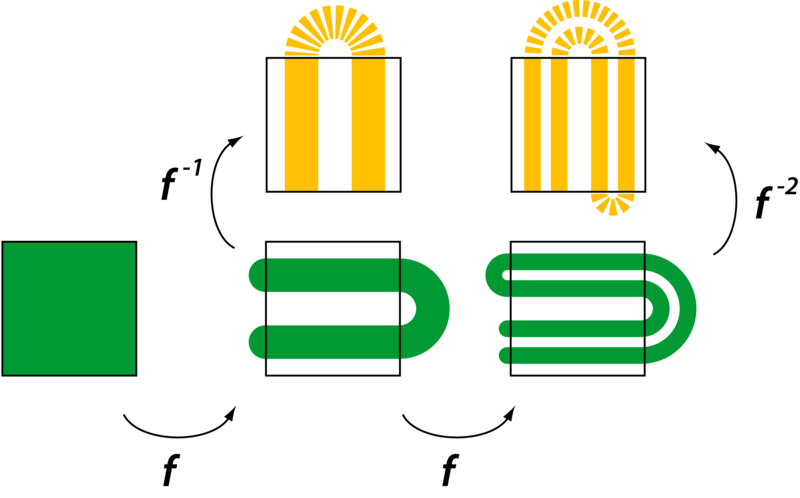
\includegraphics[width=\textwidth]{SmaleHorseshoe}
\caption{
}
\SFIG{HMV} %{SmaleHorseshoe}}
{}{SmaleHorseshoe
    }{Fig:SmaleHorseshoe}
\end{figure}

%%%%%%%%%%%%%%%%%%%%%%%%%%%%%%%%%%%%%%%%%%%%%%%%%%%%%%%%%%%%%%%%%



In Kai's thesis, he mentioned ``since the horseshoe is a diffeomorphism we need to
know both the future and the past.'' With the help of this picture I kind
of understand this.

Also I found something interesting that animate the procedure of H\'enon
map horseshoe:
\HREF{http://www.ibiblio.org/e-notes/Chaos/henon.htm}
{www.ibiblio.org/e-notes/Chaos/henon.htm}

\item[2011-07-23 PC]                                        \inCB
I had noticed Demidov's website before - you are right, these simulations
are very instructive, I have now added a remark about them to ChaosBook.
He uses a different definition for parameters $a$ and $b$ from H\'enon,
but unfortunately uses the same letters. His definition is natural if one
is interested in Julia sets, but unfortunately not the one H\'enon used,
and I always try to follow the foundational papers, rather than confusing
everybody with sly parameter redefinitions.

Can you write here the transformation between two definitions? You
need this, if you are going to use Demidov's simulations to test your
ideas.

\item[2011-07-24 CS]
Yeah I also noticed that. 
Traditional Henon map: 
\[
x'=1-a'x^2+b'y
\]
\[
y'=x
\]
Demidov's definition of Henon map:
\[
x''=a''+x^2+b''y
\]
\[
y''=x
\]
rewrite x'' as 
\[
\frac{x''}{a''}=1+\frac{1}{a''}x^2+\frac{b''}{a''}y
\]
compare with the traditional definition, we obtain the relation between them:
\[
x'=\frac{x''}{a''}
\]
\[
a'=-\frac{1}{a''}, b'=\frac{b''}{a''}
\]



\item[2011-07-22 CS] BTW, I forgot to ask the first question on the list
yesterday "In my understanding, in a non-wandering and chaotic set, any
unstable trajectory is ergodic. That means the trajectory will finally
visit any infinitesimally small volume in the the set. Right?"

\item[2011-07-23 PC]
Mhm... I wrote a suggestion what to read above, dated {\bf 2011-07-20
PC}. After rereading the discussion in ChaosBook, let me know what is
missing there...





\end{description}
